\documentclass{llncs}
%\documentclass[a4paper]{article}

\usepackage{fullpage}
\usepackage{setspace}
\usepackage{url}
\usepackage{algorithmic}
\usepackage{algorithm}
\usepackage{amsmath}
\usepackage{latexsym}

\usepackage{graphicx}
\usepackage{subfig}

\onehalfspacing

%\newtheorem{definition}{Definition}
%\newtheorem{theorem}{Theorem}
%\newtheorem{example}{Example}
\newtheorem{query}{Query}

%\newcommand{\nop}[1]{}

\setlength{\tabcolsep}{2pt}

\newcommand{\myremark}[2]{{\textbf{\marginpar{$\parallel$}(* \textit{#1:} #2 *)}}}

\title{Mapping Microblog Posts to Encyclopedia Articles}
\author{Uta L\"{o}sch \and David M\"{u}ller \and Andreas Harth}
\institute{
	Karlsruhe Institute of Technology (KIT), D-76131 Karlsruhe, Germany\\ 
	\email{uta.loesch@kit.edu},\\
	\email{david.mueller@student.kit.edu},\\
	\email{harth@kit.edu}
}
\begin{document}

\maketitle

\begin{abstract}
To facilitate understanding the meaning of a hash tag in the context of Twitter, we have developed a system which annotates hash tags based on Twitter search results with encyclopedia entities that best describe the hash tag, thus offering means of quickly grasping the meaning of the hash tag and at the same time providing starting points for further exploration of the hash tags' context. In an evaluation we show that the encyclopedia entities used for annotation represent the content in a suitable manner and that the annotations remain stable over time, i.e. when executing the same search at different times, the same entities are returned.
\end{abstract}

Keywords: Twitter, Wikipedia, DBpedia, RDF

\section{Introduction}

Twitter\footnote{\url{http://twitter.com}} is a micro-blogging service that has become very influential over the last years. The idea of micro-blogs is the same as that of blogs, except that the message length is restricted, in the case of Twitter the restriction is 140 characters. Twitter has a total of about 190 million of users who produce 65 million Twitter messages a day. Thus, Twitter represents a huge data source on the web.

On Twitter it is possible to search for messages containing a specific term or hash tag. This search returns a fixed number of most recent messages containing the search term. However, it is hard to grasp the context of the results and to get further information on the topic that was searched for. As each single Twitter message is very short and contains little information, it is necessary to parse the whole set in order to get an overview of the context(s) in which the search term is used. 

To facilitate this putting into context of the search results, we propose to annotate search results with a set of entities which reflect the content of the result feeds. These entities will not only help to understand the search terms, but also serve as a starting point for refining the search or searching for further information related to the search result. 

Furthermore, this annotation will help to understand hash tags. Hash tags are frequently used to associate messages with a specific topic, place, person or event on Twitter. For example, messages talking about what is going on at the European Semantic Web Conference 2011 will frequently be tagged with $\#eswc2011$. If a user encounters this hash tag and does not understand it, he can search for it on Twitter. However, as discussed before, to understand a search result is difficult and time-consuming. Using our approach the search will not only return messages using the tag but also a set of entities which have been detected in the search result. These entities will help the user to gain an understanding in which context the hash tag is used and what it may mean.

Finding entities matching a query, especially a query for a given hash tag is difficult due to synonyms and homonyms in the set of hash tags that are frequently used. For example, both the hash tags $\#ka$ and $\#karlsruhe$ are frequently used when talking about topics which are related to the city Karlsruhe. The tag $\#ka$ is however also used in the context of the car type Ford Ka. Thus, when searching for $\#ka$ on Twitter, messages relating to Karlsruhe will be found as well as messages related to Ford Ka. An approach which aims at finding relevant entities for a given search will have to be able to deal with these problems.

In this paper, we present a system which automatically annotates a Twitter search result with Wikipedia entities. While it would be more interesting to annotate each single Twitter message with relevant entities, Twitter messages are too short to contain much relevant information which could be used as input for the annotation tool. Thus, we chose to generate annotations for the whole search result. 

The motivation for choosing Wikipedia as entity source was that it offers a wide coverage of topics. Furthermore, automatic tools for annotating text with Wikipedia entities are readily available (see \cite{key:wikifier}).

Annotations should be stable over time, unless the topics discussed in the Twitter messages containing the search term change. In an evaluation of our approach we have tried to analyze the stability of the result.

Our contributions thus are:
\begin{itemize}
	\item an approach for finding entities which are related to a search on Twitter
	\item an implementation of our approach
	\item an evaluation of the stability and relevance of the entities found with our approach.
\end{itemize}

The rest of this paper is organized as follows: in Section~\ref{sect:relWork} we discuss related work, in Section~\ref{sect:method} we present our approach, the results of our evaluation are presented in Section~\ref{sect:eval}, before we conclude in Section~\ref{sect:conclusion}.

\section{Related Work}
\label{sect:relWork}

Bringing Semantic Web technologies and Semantic Web technologies together, has been proposed several times.

The SemanticTweet\footnote{\url{http://semantictweet.com}} service is a tool which allows for the generation of a FOAF file describing one's network of followers and friends on Twitter. Thus, an automatic way of mapping the Twitter social network to semantic data is made available.

The challenge task in the WePS-3 Online Reputation Management Task\cite{key:clef} requires systems to detect mentions of company names in Twitter messages.
The corpus contains evaluation results solicited via Mechanical Turk.
In contrast to the WePS-3 task, we associate generic hash tags to Wikipedia/DBpedia concepts.
@@@even with hashtags we have ambiguity, how would be map Twitter message containing the keyword ``apple''?

Softic et al \cite{key:softic} have developed a framework and system for mining
data from social networks. They have instantiated their system to analyze data from Twitter. In their system, they collect data from one or several users. The system by Passant et al. \cite{key:smob} is used for transforming twitter data to semantic data. The triplified data can then be analysed using SPARQL. They propose that the result data could be enriched using entities from other Linked Open data vocabularies like dbpedia\footnote{\url{http://dbpedia.org}} or GeoNames\footnote{\url{http://www.geonames.org}}, but they do not provide a method for achieving this.
Wagner \cite{key:clauwa} proposes to use aggregations of social awareness streams for knowledge extraction.
As such, our approach is closely related.
Stankovic et al. \cite{key:stanko} propose to use the Zemanta\footnote{\url{http://developer.zemanta.com/}} keyword extraction API to detect topics of single Twitter messages.
% from stakovic et al.
%In order to make tweets more searchable and make them useful for the described
%scenario one would need to have represent them in a structured format and associate
%those tweets with the topics that refer to. As a basic approach we process the text of
%the tweets using Zemanta16 keyword extraction API. This approach gives DBPedia
%concepts related to a tweet, but is useful only on a limited number of tweets directly
%mentioning a particular topic. In the example data set we produced from ESWC2010,
%tweet topics are represented using dc:subject property.

Instead of mining single messages which provide little signal to the extraction algorithm we use an aggregation of messages (as proposed by Wagner \cite{key:clauwa}) as input to the extraction component.
The system we use for mapping text to Wikipedia entities has been proposed by Milne and Witten \cite{key:wikifier}. 
The so-called Wikifier maps text to Wikipedia pages, which in turn directly map to DBpedia URIs.
%uhe: System beschreiben
Kinsella et al. \cite{key:kinsella} use hyperlinks in posts to derive a richer representation of those posts.
We too use external data to augment the set of Twitter messages supplied to the Wikifier system.

Passant et al. \cite{key:smob} have proposed a data model for making Twitter data available on the Semantic Web. They propose a data model which allows for the association of URIs with users, microblogs and microposts. To this end, SIOC and FOAF vocabularies are used and extended. Specifically, the new concepts \emph{Microblog} and \emph{MicroBlogPost} are introduced. Additionally, they propose the use of so-called semantic hash tags. The idea is to use URIs as hash tags (e.g. \emph{\#geo:Paris\_France}). It becomes thus possible to link microposts to entities in the Linked Open Data cloud via these semantic hash tags. 
In contrast to this approach we do not require users to change their behavior by requiring them to use another type of hash tags. Instead, our method finds Linked Open Data entities which are related to the query automatically.

Softic et al \cite{key:softic} have developed a framework and system for mining data from social networks. They have instantiated their system to analyze data from Twitter. In their system, they collect data from one or several users. The system by Passant et al. \cite{key:smob} is used for transforming Twitter data to semantic data. The triplified data can then be analysed using SPARQL. They propose that the result data could be enriched using entities from other Linked Open data vocabularies like dbpedia\footnote{\url{http://dbpedia.org}} or GeoNames\footnote{\url{http://www.geonames.org}}, but they do not provide a method for achieving this.




\section{Method Overview}
\label{sect:method}

The goal of our method is to, given a search query $q$ as input, provide the user with an RDF\footnote{\url{http://www.w3.org/RDF/}} document describing the search result $R$, i.e. the most recent messages that match the query, the authors of these messages and the most relevant entities $E$ for this result.

The architecture of our proposed system is shown in Figure~\ref{fig:arch}. Upon receipt of a query four steps are performed. In the following we will illustrate these steps using the example of a search for the hash tag $\#ka$, a hashtag which is frequently used to describe posts related to the city of Karlsruhe, Germany.

\begin{figure}[htb]
  \centering
  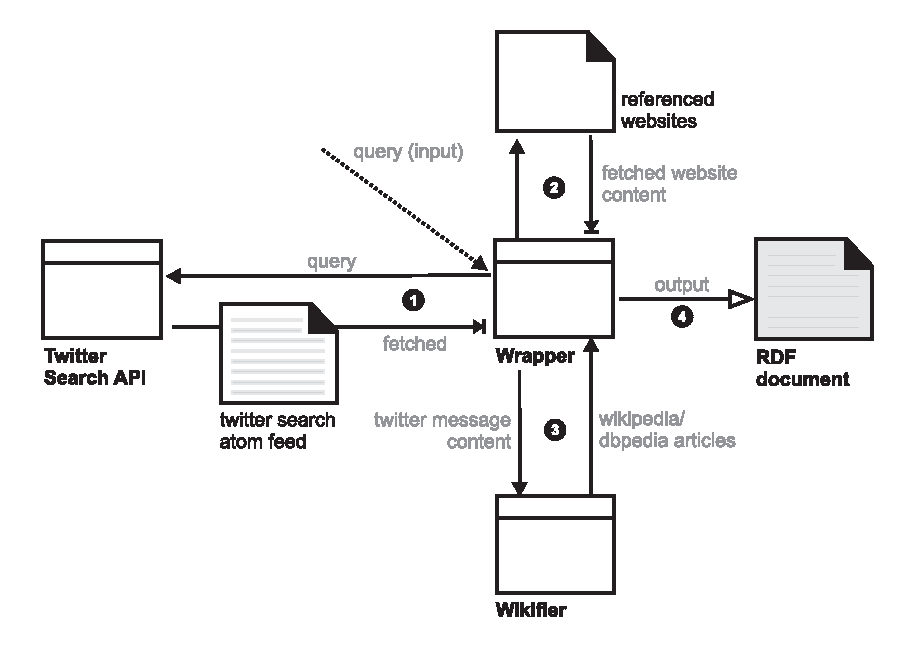
\includegraphics[width=.6\linewidth]{architecture}
  \caption{System Architecture}
  \label{fig:arch}
\end{figure}

\begin{enumerate}
	\item In a first step, the most recent search results for the query are
	obtained.\newline In our example, calling the Wrapper with query $\#ka$ will
	return a document containing all most recent Twitter posts whose content matched the search string $\#ka$ and their meta information.

An example for a single retrieved post is the following: ''\texttt{Just
returned from a wonderful holiday in \#ka.
\url{http://www.karlsruhe.de/stadt/tourismus.en} @KarlsruheTweets}'', posted by
Twitter user \texttt{sample\_user\_12345}; geo coordinates and the date
the message has been posted be furthermore known.
  
  \item In a second (optional) step hyperlinks posted in messages of the fetched
  feed are followed, content of the referenced website is fetched and processed by the Wrapper. The idea is to acquire additional content which is used as additional signal when searching for entities. We have thought of other methods for enriching the result, like searching for other messages posted by users which have posted messages in the result set. However, these alternative methods are more likely to introduce noise in the signal which is used for obtaining relevant entities.
  
In our example, the message contains a link to
\url{http://www.karlsruhe.de/stadt/tourismus.en}, the official homepage of the
tourist office of the city of Karlsruhe. Dereferencing this URL and grabbing the
text found at the link gives us the following text: ''\texttt{Karlsruhe, where
paths converge - a legendary city in the sunny south-west of Germany, famed for its fan-shaped historic street plan, where margraves reigned in times past, and German joie de vivre reigns today.}''
	
	\item In a third step entities matching the search result are retrieved. The content of the Twitter messages that matched the search query and, if available, the content of referenced websites is merged to a single input string and used as input for the annotation. The result of this step is a list of matching articles of the English Wikipedia.

In our example, the contents of all posts related to the search term '\#ka' are merged with the retrieved external website content. Thus, the post obtained from step 1 would be matched with the website content obtained in step 2 into a single input stream: \texttt{Just returned from a wonderful holiday in \#ka. \url{http://www.karlsruhe.de/stadt/tourismus.en} @KarlsruheTweets. Karlsruhe, where paths \newline converge - a legendary city in the sunny south-west of Germany, famed for its \newline fan-shaped historic street plan, where margraves reigned in times past, and German \newline joie de vivre reigns today.} 
This string is appended to the Twitter content and the external content of all other posts in the result.

In the example, we would expect to find entities which are related to Karlsruhe, like Karlsruhe, Germany or the Karlsruhe\_Institute\_of\_Technology.

	\item	Finally, an RDF document is generated representing the search results and the annotations.  
	
	Continuing our example, the output RDF document contains the following triples
	to reference the DBPedia mappings:\newline
	\texttt{<rdf:Description rdf:about=""/>}\newline
	\texttt{<rdfs:seeAlso rdf:resource="http://dbpedia.org/resource/Karlsruhe"/>}\newline
	\texttt{<rdfs:seeAlso rdf:resource="http://dbpedia.org/resource/Germany"/>}\newline
	\texttt{<rdfs:seeAlso rdf:resource="http://dbpedia.org/resource/\newline
	Karlsruhe\_Institute\_of\_Technology"/>}\newline
	\texttt{</rdf:Description>}\newline
	The Twitter posts matching the search term \#ka are all described in the output document. As an example, the description for the initially given post results in the following RDF output:
	
	\texttt{<rdf:Description rdf:about="http://km.aifb.kit.edu/services/twitterwrap/statuses/\newline
	show/1234567890\#id">\newline
	<foaf:page rdf:resource="http://twitter.com/sample\_user\_12345/statuses/1234567890"/>\newline
	<dc:date>2011-02-23T12:00:00Z</dc:date>\newline
	<geo:lat>49.010239</geo:lat>\newline 
	<geo:long>8.411879</geo:long>\newline
	<foaf:maker rdf:resource="http://km.aifb.kit.edu/services/twitterwrap/users/\newline
	show?screen\_name=sample\_user\_12345\#id"/>\newline 
	<dc:description>\newline
	Just returned from a wonderful holiday in \#ka.
	\url{http://www.karlsruhe.de/stadt/tourismus.en} @KarlsruheTweets\newline
	</dc:description>\newline
	</rdf:Description>\newline}
\end{enumerate}
\myremark{Uta}{Gibt es was, was man zu Dublin Core zitieren kann?}

\section{Implementation}

In the Twitter Search Wrapper\footnote{Available at \url{http://km.aifb.kit.edu/services/twittersearchwrap/}} we provide an implementation of our approach.

The implementation is based on a set of existing components: Twitter search results are obtained by using the Twitter search API\footnote{\url{http://dev.twitter.com/doc/get/search}}. The result is a feed containing the 100 most recently published Twitter messages, which are publicly visible and match the query, and their authors. The messages themselves are described by their content, publishing date, authors
and optionally a geographic location.

The optional step of dereferencing URLs which are posted in messages contained
in the result set can be triggered using the option \texttt{extern=true}. To keep the input size for the next steps manageable, we do not use the whole content of the referenced sites but only the first 50 words.

The Wikifier \cite{key:wikifier} is used for obtaining content annotations. This tool takes a text as input and returns a set of Wikipedia entities which are relevant for the analyzed text.

The RDF document describes the result by means of the popular vocabularies FOAF \cite{key:foaf}, Dublin Core\footnote{\url{http://dublincore.org/documents/dcmi-terms/}}, the Basic Geo Vocabulary \cite{key:geo}. The annotations are added to the search result using \texttt{rdf:seeAlso} links to DBpedia entities \cite{key:dbpedia} which are obtained by a direct transformation of the Wikipedia entities' URLs. DBpedia has been chosen as these entities allow for a more coherent presentation of the content in the context of RDF.

\myremark{Uta}{David, kannst Du das Ausgabeformat noch etwas ausf�hrlicher beschreiben? Welche Informationen werden genau dargestellt, welche Relationen werden wof�r verwendet?}

%The implemented system\footnote{\url{http://km.aifb.kit.edu/services/twittersearchwrap/}} (further called Twitter Search Wrapper) is called with a query representing
%the Twitter search term and returns a RDF}
%document semantically describing the most recent Twitter messages matching the
%given query. The returned RDF document furthermore contains a mapping of the
%query to Encyclopedia articles which based on the content published by users that most recently used the search
%term in their posts maps to articles best describing the content of Twitter
%messages related to the term. An overview of the System Architecture is given in Figure
%\ref{fig:arch}.\newline 
%Taking a more detailed look, methods performed by the
%Twitter Search Wrapper can be grouped into five sequential steps (see Figure
%\ref{fig:arch}). We will follow those steps along a simple example, using
%\#ka (a hashtag frequently used to describe posts related to the city of
%Karlsruhe, Germany) as search term for the Twitter Search wrapper.


%\begin{enumerate}
%  \item 
%In a first step the Twitter Search Wrapper fetches the atom feed (XML Data)
%generated by the Twitter Search
%API\footnote{\url{http://dev.twitter.com/doc/get/search}} for a given
%search query. The generated feed contains the data of the 100 most recently published
%publicly visible Twitter messages and their authors which match the search query.
%The messages themselves are described by their content, publishing date, authors
%and optionally a geographic location.\linebreak\linebreak
%In the given example, calling the Wrapper with query '\#ka' will return a
%document containing all most recent Twitter posts and their meta information
%whose content matched the search string '\#ka'. Taking a closer look, a single
%retrieved post might have the following content: \newline\linebreak 
%\texttt{Just returned from a wonderful holiday in \#ka.
%\url{http://www.karlsruhe.de/stadt/tourismus.en} @KarlsruheTweets}
%\linebreak
%\item
%In a second (optional) step hyperlinks posted in messages of the fetched
%feed are followed, content of the referenced website's body is fetched and
%processed to the Wrapper. This option is triggered calling the Twitter Search
%Wrapper with attribute extern=true.\newline
%\linebreak
%Following the initial example, the given sample post contained a link to
%\url{http://www.karlsruhe.de/stadt/tourismus.en}, the official homepage of the tourist office of the city of Karlsruhe, which contains the following
%text:\newline
%\linebreak
%''\texttt{Karlsruhe, where paths converge - a legendary city in the sunny
%south-west of Germany,\newline famed for its fan-shaped historic street plan,
%where margraves reigned in times past,\newline and German joie de vivre reigns
%today.}''\newline\linebreak
%The text is fetched and returned to the Wrapper. The same accounts for
%content of all other websites that were referenced in the list of posts matching
%the query \#ka.\newline
%\item
%The Wrapper now calls the Wikifier (see \cite{key:wikifier}). Content of
%the Twitter messages that matched the search query and optional content of their
%referenced websites is merged to a single input string which is used as input for the Wikifier. The service
%returns a list of matching articles of the English
%Wikipedia. Optionally the wrapper can be initially called with attribute lang=de
%to trigger mapping to the German Wikipedia.\newline\linebreak
%In the given example, content of all posts related to the search term '\#ka' is
%merged with retrieved external website content. Taking a closer look at the
%single post we merge its content and content of its referenced website to
%a single string:\newline\linebreak
%\texttt{Just returned from a wonderful holiday in \#ka.
%\url{http://www.karlsruhe.de/stadt/tourismus.en} @KarlsruheTweets. Karlsruhe,
%where paths converge - a legendary city in the sunny\newline south-west of
%Germany, famed for its fan-shaped historic street plan, where margraves\newline
%reigned in times past, and German joie de vivre reigns today.}\newline\linebreak
%This string is appended to Twitter content and external content of all other
%posts that have been retrieved in this way matching the initial query \#ka and
%used as input for the Wikifier.\newline
%  \item
%The Wikifier now maps the input string to relevant Wikipedia articles. A
%detailed description of this process can be found under \cite{key:wikifier}. 
%The list of matching Wikipedia articles is finally returned to the
%Wrapper.\newline\linebreak
%In the given example, a desired mapping of the contents of posts related to the
%hashtag \#ka and mapping for the hashtag \#ka as such, would preferably be a
%mapping to Wikipedia articles describing content related to Karlsruhe. We just
%assume this results in mappings to the articles for Karlsruhe, Germany and the
%Karlsruhe\_Institute\_of\_Technology.\newline
%  \item
%The Wrapper finally generates a RDF document using popular ontologies
%(foaf\footnote{http://xmlns.com/foaf/spec/},
%dublincore\footnote{http://dublincore.org/documents/dcmi-terms/}, geo\footnote{http://www.w3.org/2003/01/geo}) to describe the data related to the
%returned Twitter messages and their content using 'rdfs:seeAlso' triples to link
%the document to DBPedia\footnote{\url{http://dbpedia.org/About}} URIs (converted
%output of the Wikifier) that have been mapped to the documents content.
%At this point DBPedia is chosen as referenced encyclopedia, because its
%semantic nature and description of Wikipedia article content contributes to a
%coherent semantic description in the RDF document. \newline\linebreak Coming
%back to the example, the output RDF document contains the following triples to reference the
%DBPedia mappings:\newline\linebreak \texttt{<rdfs:seeAlso
%rdf:resource="http://dbpedia.org/resource/Karlsruhe"/>}\newline
%\texttt{<rdfs:seeAlso
%rdf:resource="http://dbpedia.org/resource/Germany"/>}\newline
%\texttt{<rdfs:seeAlso rdf:resource="http://dbpedia.org/resource/\newline
%Karlsruhe\_Institute\_of\_Technology"/>}\newline\linebreak 
%The twitter posts matching the search term \#ka are all described in the output
%document. As an example, the description for the initially given post might
%result in the following RDF output:\newline\linebreak
%\texttt{<rdf:Description
%rdf:about="http://km.aifb.kit.edu/services/twitterwrap/statuses/\newline
%show/1234567890\#id">\newline <foaf:page
%rdf:resource="http://twitter.com/sample\_user\_12345/statuses/1234567890"/>\newline
%<dc:date>2011-02-23T12:00:00Z</dc:date>\newline
%<geo:lat>49.010239</geo:lat>\newline <geo:long>8.411879</geo:long>\newline
%<foaf:maker
%rdf:resource="http://km.aifb.kit.edu/services/twitterwrap/users/\newline
%show?screen\_name=sample\_user\_12345\#id"/>\newline <dc:description>\newline
%Just returned from a wonderful holiday in \#ka.
%\url{http://www.karlsruhe.de/stadt/tourismus.en} @KarlsruheTweets\newline
%</dc:description>\newline
%</rdf:Description>\newline}
%\end{enumerate}

\section{Experiments and Evaluation}
\label{sect:eval}

\subsection{Setup}

Topics trending worldwide and in Germany at Twitter retrieved on February 24th
17:20h (GMT) are listed in Table \ref{tbl:terms}. These trending topics will
constitute a basis of input search terms for our evaluation of the Twitter
Search Wrapper.

\begin{table}[ht*]
\centering
\begin{tabular}{ |l|l| }
\hline
\textsc{Trending Topic} & \textsc{Location}  \\
\hline
\#goodlucknickj & Worldwide \\
\#smalljoys & Worldwide \\
\#thingsthedevilinvented & Worldwide \\
Adam Wainwright & Worldwide \\
CatchPetrovaFire & Worldwide \\
Gadafi & Worldwide \\
Libia & Worldwide \\
Precious Minaj & Worldwide \\
Tommy John & Worldwide \\
\hline
\#gaddafi & Germany \\
\#guttenberg & Germany \\
\#libya & Germany \\
Doktorarbeit & Germany \\
Gef\"{u}hl & Germany \\
Lion & Germany \\
MBP & Germany \\
Thunderbolt & Germany \\
Vorratsdatenspeicherung & Germany \\
\hline
\end{tabular}
\caption{Search terms}\label{tbl:terms}
\end{table}

\subsection{Measures}

The goal of our evaluation was to examine the stability of the entity
annotations over time. To achieve this, we have repeatedly executed the same set
of queries and saved the returned data. Two methods for this data acquisition
were identified: \begin{definition}[Data Acquisition Methods]
\begin{itemize}
\item {\bf Temporal Sliding Window}\newline The query is executed and the n
most recent results are retrieved every t minutes. The Temporal Sliding Window
method may lead to duplicate messages in the retrieved documents, but needs to
handle much less data and allows for an analysis over larger time frames.
\item {\bf k-item Sliding Window}\newline  The k-item Sliding Window methods
retrieves all messages that match the query exactly one time. Each time k new messages are
available matching the given query a document containing those k messages
is retrieved. This method can lead to high data volume and needs constant
monitoring of recently posted messages matching the search term.
\end{itemize}
\end{definition}

We considered the trending topics on Twitter a good set of input queries for
our evaluation approach. Trending topics often cover a variety of recently
talked about topics which due to its recent nature may be of high interest for
further processing. Using the retrieved trending topics given in Table
\ref{tbl:terms} as input queries for the evaluation, the set of queries was executed twice per hour using the Temporal Sliding Window method for data acquisition in a 24 hour time frame starting from the moment the topics were identified as trending topics. We chose the Temporal Sliding Window method for data acquisition because of the expected data volume generated by trending topics as search terms and the long term nature of our evaluation approach. We have then evaluated the results
with respect to several measures:

\begin{definition}[Evaluation Measures]
Given disjoint result sets $R_1,\ldots,R_n$ for a query $q$ obtained at times $t_1,\ldots,t_n$ and annotated with sets of entities $E_1,\ldots,E_n$, we define:
\begin{itemize}
	\item The average disjoint time $adt$ for a query is the average time that has to lie between two result sets in order to obtain disjoint results: $$adt(q)=\frac{\sum_{i=1}^{n}t_{i+1}-t_i}{n-1}$$
	A high $adt(q)$ means that new messages that match the query $q$ are not generated very often. If new messages matching the query $q$ are frequently published, then the $adt(q)$ is low.
	\item The global stability $gs$ of the results shows how stable the whole set of entity terms for a query is. It is defined as: $$gs(q)=\frac{|\bigcap_{i=1}^{n}E_i|}{|\bigcup_{i=1}^{n}E_i|}$$
	A value of $gs(q)$ of $1$ means that the set of entities is the same at each point in time $t_i$. On the other hand, a value of $0$ means that at least two of the sets of entities, with which the results were annotated, are disjoint.
	\item The time stability $ts$ for a query $q$ at time $t_i$ is the fraction of entities which are unchanged between the result set at $t_{i-1}$ and $t_i$:
	$$ts(q,t_i)=\begin{cases} |E_i| & i=1 \\
														\frac{|E_{i-1}\cap E_i|}{|E_{i-1}\cup E_i|} & i>1\end{cases}$$
	Here again, a value of $1$ means that the two sets of entities are identical, a value of $0$ means they are disjoint.
	\item The stability for a single term is defined as the fraction of result sets for a query $q$ in which it occurs: 
$$sts(q,t)=\frac{|\{i|t\in E_i\}|}{n}$$
	If the value of $sts$ is $1$ the term occurs in all of the result sets for the query, if it is close to $0$ it occurs in few result sets.
\end{itemize}
\end{definition}

\subsection{Results}

\myremark{Uta}{In der Evaluationstabelle sollte dann auf jeden Fall noch dabei stehen, wie viele Resultsets wir zu den einzelnen Queries haben}

\subsection{Discussion}

@@@highlight the remarkable outcomes
@@@what is did we learn from the results?


\section{Conclusion}
\label{sect:conclusion}

@@@ not possible to map one hashtag to a single dbpedia concept: \#ka may be used for Karlsruhe or Ford Ka

@@@ tricky to deal with different languages - wikifier (or any nlp technique) is language dependent, but the trending topics may be commented on in a variety of languages

@@@ how to select external data (parse text from HTML, which part of web page to select - boilerplate stuff might spoil the results (reference blog cleansing paper

\bibliographystyle{abbrv}
\bibliography{bib}

\end{document}
